\documentclass[12pt,a4paper,twoside,openright]{book}

% ============================================
% PAQUETES ESENCIALES
% ============================================

% Codificación y lenguaje
\usepackage[utf8]{inputenc}
\usepackage[spanish,es-tabla,es-nodecimaldot]{babel}
\usepackage[T1]{fontenc}

% Geometría de página (margen izquierdo mayor para encuadernación)
\usepackage[left=3cm,right=2.5cm,top=2.5cm,bottom=2.5cm]{geometry}

% Gestión bibliográfica IEEE
\usepackage[backend=biber,style=ieee,citestyle=numeric-comp,sorting=none]{biblatex}
\addbibresource{referencias.bib}

% Gráficos y figuras
\usepackage{graphicx}
\graphicspath{{imagenes/}}
\usepackage{float}
\usepackage[font=small,labelfont=bf]{caption}
\usepackage{subcaption}

% Tablas profesionales
\usepackage{booktabs}
\usepackage{longtable}
\usepackage{multirow}
\usepackage{array}
\usepackage{tabularx}

% Matemáticas
\usepackage{amsmath,amssymb,amsthm}

% Interlineado
\usepackage{setspace}
\onehalfspacing

% Encabezados y pies de página
\usepackage{fancyhdr}
\pagestyle{fancy}
\fancyhf{}
\fancyhead[LE,RO]{\thepage}
\fancyhead[RE]{\leftmark}
\fancyhead[LO]{\rightmark}
\renewcommand{\headrulewidth}{0.4pt}

% Hipervínculos y referencias cruzadas (DEBE IR AL FINAL)
\usepackage[hidelinks,colorlinks=true,linkcolor=black,citecolor=blue,urlcolor=blue]{hyperref}
\usepackage{bookmark}

% Formato de capítulos
\usepackage{titlesec}
\titleformat{\chapter}[display]
  {\normalfont\huge\bfseries}{\chaptertitlename\ \thechapter}{20pt}{\Huge}
\titlespacing*{\chapter}{0pt}{-50pt}{40pt}

% Color para resaltar
\usepackage{xcolor}

% ============================================
% INFORMACIÓN DEL DOCUMENTO
% ============================================
\title{Implementación de un Sistema de Automatización Inteligente del Proceso de Calificación y Generación de Proyectos de Resolución de Expedientes mediante Modelos de Lenguaje}
\author{Deglan Jesus Rivas Romero}
\date{Lima, 22 de enero del 2026}

% Metadatos PDF
\hypersetup{
    pdftitle={Implementación de un Sistema de Automatización Inteligente del Proceso de Calificación y Generación de Proyectos de Resolución de Expedientes mediante Modelos de Lenguaje},
    pdfauthor={Deglan Jesus Rivas Romero},
    pdfsubject={Trabajo de Suficiencia Profesional - Ingeniería Mecatrónica},
    pdfkeywords={rendición de cuentas, transparencia, gestión pública, SIRCTGE, corrupción, Perú},
}

% ============================================
% INICIO DEL DOCUMENTO
% ============================================
\begin{document}

% ============================================
% PORTADA
% ============================================
\begin{titlepage}
    \centering
    \vspace*{1cm}

    % Logo PUCP
    
\includegraphics[width=0.3\textwidth]{image1.jpeg}\\[1.5cm]

    {\scshape\Large Pontificia Universidad Católica del Perú\\[0.3cm]
    Facultad de Ciencias e Ingeniería\\[0.5cm]}

    \vspace{1.5cm}

    {\huge\bfseries Implementación de un Sistema de Automatización Inteligente del Proceso de Calificación y Generación de Proyectos de Resolución de Expedientes mediante Modelos de Lenguaje\\[1.5cm]}

    {\Large\itshape Trabajo de Suficiencia Profesional\\[0.3cm]
    para optar el título profesional de\\[0.3cm]
    Ingeniero Mecatrónico\\[1.5cm]}

    {\Large\textbf{Autor:}\\
    Deglan Jesus Rivas Romero\\[1cm]}

    {\Large\textbf{Asesor:}\\
    Felix Melchor Santos Lopez\\[2cm]}

    \vfill

    {\large Lima, Perú\\
    22 de enero del 2026}

\end{titlepage}

% ============================================
% PÁGINAS PRELIMINARES (numeración romana)
% ============================================
\frontmatter
\pagenumbering{roman}

% ============================================
% RESUMEN
% ============================================
\chapter*{Resumen}
\addcontentsline{toc}{chapter}{Resumen}

[TODO] pendiente de completar al final del curso

\textbf{Palabras clave:} [TODO] pendiente de completar al final del curso.

% ============================================
% DEDICATORIA
% ============================================
\chapter*{Dedicatoria}
\addcontentsline{toc}{chapter}{Dedicatoria}

\vspace*{5cm}
\begin{flushright}
\itshape
A mis padres, por su apoyo incondicional.\\[0.5cm]
% A mí.
\end{flushright}

% ============================================
% AGRADECIMIENTOS
% ============================================
\chapter*{Agradecimientos}
\addcontentsline{toc}{chapter}{Agradecimientos}

Agradezco a mi familia por los valores y apoyo incondicional.

Agradezco a mi equipo de trabajo por su colaboración y orientación constante.

% A mí por la dedicación invertida.

% ============================================
% ÍNDICES
% ============================================
\tableofcontents

\listoftables
\addcontentsline{toc}{chapter}{Índice de tablas}

\listoffigures
\addcontentsline{toc}{chapter}{Índice de figuras}

% ============================================
% CONTENIDO PRINCIPAL (numeración arábiga)
% ============================================
\mainmatter
\pagenumbering{arabic}

% ============================================
% CAPÍTULO I: PROBLEMÁTICA
% ============================================
\chapter{Problemática}
\label{cap:problematica}

\section{Descripción del problema}
\label{sec:descripcion-problema}

El Jurado Nacional de Elecciones (JNE), como máximo órgano de administración de justicia electoral en el Perú, enfrenta desafíos significativos derivados de la escasa automatización de sus plataformas jurídicas y la ausencia de estandarización en numerosos procesos operativos. Esta situación ocasiona un uso ineficiente de recursos institucionales, traducido en mayor inversión de tiempo, presupuesto y esfuerzo humano, además de incrementar la vulnerabilidad a errores en procedimientos críticos para la democracia nacional.

\subsection{Contexto de las elecciones 2026}

Las Elecciones Generales (EG) 2026 representan un hito histórico para el sistema electoral peruano, al coincidir por primera vez en dos décadas con las Elecciones Regionales y Municipales (ERM). Este evento excepcional ---que ocurre cada 20 años debido a que las EG se realizan cada 5 años y las ERM cada 4 años--- ha sido calificado por la Oficina Nacional de Procesos Electorales (ONPE) como ``las elecciones más complejas de la historia'' del país \cite{onpe2022erm}.

La magnitud del proceso electoral 2026 se evidencia en las cifras: a nivel nacional se elegirán 198 autoridades, incluyendo presidente, 2 vicepresidentes, 130 diputados, 60 senadores y 5 parlamentarios andinos. Simultáneamente, las ERM contemplarán la elección de 25 gobernaciones regionales, 196 alcaldías provinciales y 1696 alcaldías distritales \cite{elcomercio2025erm}. Este escenario se complejiza aún más por el récord histórico de participación política: para las ERM 2026 se han inscrito 150 organizaciones políticas ---55 partidos y 95 movimientos---, superando ampliamente las 147 organizaciones que participaron en las ERM 2022, cuando se eligieron aproximadamente 13,000 autoridades \cite{jne2025candidatos}.

Román Campos, integrante del Gabinete de Asesores del JNE, proyecta que ``estamos hablando de aproximadamente medio millón de candidatos que podrían, potencialmente, presentarse'' \cite{jne2025candidatos}, estimación que se sitúa entre 500,000 y 700,000 candidatos considerando ambos procesos electorales simultáneos. Esta magnitud sin precedentes representa un desafío operativo sustancial para las capacidades actuales del sistema electoral.

\subsection{Restricciones presupuestales}

El contexto presupuestal agrava significativamente la situación. Para el año fiscal 2025, el JNE solicitó S/ 864 millones, pero el Ministerio de Economía y Finanzas (MEF) asignó inicialmente solo S/ 500 millones, representando un recorte de aproximadamente 42\% \cite{convoca2025presupuesto}. En conjunto, el Sistema Electoral conformado por el JNE, ONPE y Registro Nacional de Identificación y Estado Civil (RENIEC) proyecta necesitar casi S/ 4,000 millones para gestionar adecuadamente los procesos electorales de 2026 \cite{rpp2025elecciones}.

Esta brecha presupuestal subraya la necesidad crítica de optimizar recursos mediante soluciones tecnológicas que incrementen la eficiencia operativa sin comprometer la calidad del proceso de fiscalización electoral.

\subsection{Proceso actual de calificación de inscripciones}

El procedimiento vigente para la inscripción de listas de candidatos, ilustrado en la Figura~\ref{fig:flujo-sin-eleccia}, comprende las siguientes etapas:

\begin{enumerate}
    \item El personero legal de la organización política accede a la plataforma DECLARA+ del JNE.
    \item Registra la solicitud de inscripción y carga documentación oficial de la organización.
    \item Completa las Hojas de Vida correspondientes a cada candidato propuesto.
    \item El sistema genera automáticamente un expediente digital en el Sistema Integrado Judicial Electoral (SIJE).
    \item Los abogados especializados del JNE califican manualmente cada expediente, verificando el cumplimiento de requisitos legales establecidos en la normativa electoral.
    \item Se elabora un proyecto de resolución con uno de tres resultados posibles:
    \begin{itemize}
        \item \textbf{ADMISIBLE}: La lista cumple todos los requisitos y se aprueba su inscripción.
        \item \textbf{INADMISIBLE}: Existen observaciones subsanables; la organización dispone de 3 días hábiles para corregir las deficiencias.
        \item \textbf{IMPROCEDENTE}: La solicitud presenta deficiencias no subsanables y se rechaza definitivamente.
    \end{itemize}
\end{enumerate}

\begin{figure}[H]
    \centering
    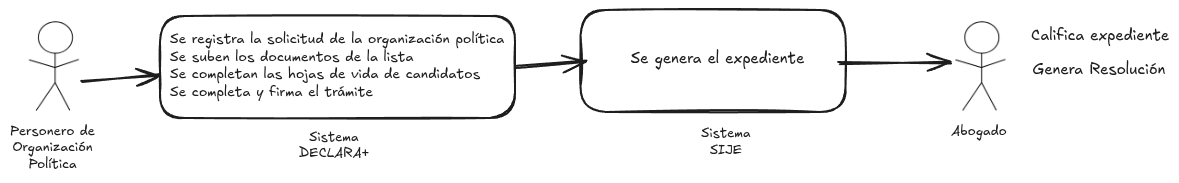
\includegraphics[width=0.95\textwidth]{flujo_sin_eleccia.png}
    \caption{Proceso manual de calificación de expedientes de inscripción de listas}
    \label{fig:flujo-sin-eleccia}
\end{figure}

Este procedimiento, completamente manual en su fase de calificación jurídica, presenta vulnerabilidades significativas ante el volumen extraordinario de expedientes proyectado para 2026. La revisión exhaustiva de documentos extensos ---como planes de gobierno que pueden superar cientos de páginas--- exige capacidades humanas que se ven sobrecargadas, incrementando el riesgo de errores por omisión, inconsistencias en la aplicación de criterios de evaluación y demoras en los plazos de calificación establecidos por el calendario electoral.

\subsection{Propuesta: Sistema EleccIA}

Ante esta problemática, el presente Trabajo de Suficiencia Profesional propone el desarrollo del sistema EleccIA, una herramienta de apoyo a la calificación jurídica que integra técnicas de inteligencia artificial para asistir a los profesionales del JNE en la evaluación de expedientes de inscripción. La Figura~\ref{fig:flujo-con-eleccia} ilustra el proceso optimizado mediante esta solución tecnológica.

\begin{figure}[H]
    \centering
    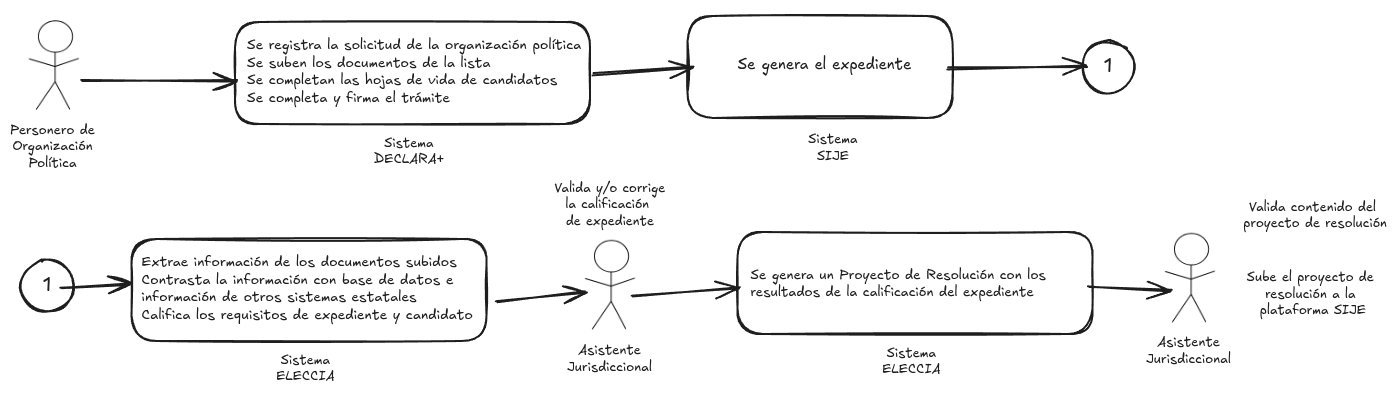
\includegraphics[width=0.95\textwidth]{flujo_con_eleccia.png}
    \caption{Proceso asistido de calificación mediante el sistema EleccIA}
    \label{fig:flujo-con-eleccia}
\end{figure}

Es fundamental enfatizar que EleccIA se concibe como una \textit{herramienta de apoyo}, no como un sistema de decisión autónoma. La revisión y validación final de cada expediente permanece bajo responsabilidad exclusiva de los profesionales del derecho del JNE, preservando el criterio humano especializado en la interpretación normativa y la garantía del debido proceso electoral. El sistema proporciona análisis preliminares, detecta inconsistencias potenciales y organiza información, permitiendo que los abogados concentren su experticia en casos que requieren interpretación jurídica compleja.

Esta aproximación busca maximizar la eficiencia del proceso sin comprometer la rigurosidad técnico-jurídica que caracteriza la función del JNE como garante de la legalidad electoral en el Perú.

\section{Objetivos del trabajo}
\label{sec:objetivos}

\subsection{Objetivos generales}
\label{subsec:objetivos-generales}

Desarrollar e implementar un sistema web de apoyo para la calificación de expedientes electorales y generación automatizada de resoluciones en el Jurado Nacional de Elecciones del Perú, mediante el procesamiento de información pública y técnicas de inteligencia artificial, con el propósito de optimizar los tiempos de respuesta y garantizar resultados de alta confiabilidad.

\subsection{Objetivos específicos}
\label{subsec:objetivos-especificos}

\begin{enumerate}
    \item Identificar y documentar los requisitos funcionales y no funcionales del sistema EleccIA mediante técnicas de ingeniería de requisitos aplicadas al contexto del proceso de calificación de expedientes electorales.

    \item Diseñar la arquitectura del sistema, incluyendo la especificación de componentes del backend, el modelado de la base de datos y los prototipos de interfaz de usuario (mockups) del frontend.

    \item Ejecutar pruebas de software en múltiples niveles (unitarias, de integración y de estrés) para validar la funcionalidad, estabilidad y rendimiento del sistema previo a su puesta en producción.

    \item Realizar el despliegue del sistema en ambiente productivo e implementar mecanismos de trazabilidad y monitoreo para la detección, registro y gestión de errores operacionales.

    \item Construir un tablero de control (dashboard) que visualice las métricas clave sobre el uso del sistema EleccIA, permitiendo el análisis del comportamiento y la adopción por parte de los usuarios finales.

    \item Determinar los costos de implementación y operación del sistema, así como calcular el retorno de inversión (ROI) mediante la comparación con el proceso tradicional de calificación manual de expedientes.
\end{enumerate}

\section{Soluciones existentes}
\label{sec:soluciones-existentes}

La implementación de inteligencia artificial en sistemas de gestión documental y validación de expedientes ha experimentado un desarrollo significativo en el ámbito judicial y electoral de América Latina durante la última década. Esta sección examina las soluciones tecnológicas más relevantes que han abordado problemáticas similares a las que enfrenta el sistema electoral peruano, con especial énfasis en la automatización de procesos de revisión documental, extracción de información y validación de datos.

\subsection{Sistemas de gestión judicial automatizada}

\subsubsection{Proyecto Victor (Supremo Tribunal Federal de Brasil)}

El Supremo Tribunal Federal de Brasil desarrolló el Proyecto Victor como respuesta a la necesidad de procesar volúmenes masivos de documentación judicial \cite{stf2021victor}. Este sistema representa uno de los casos de éxito más destacados en la aplicación de inteligencia artificial al ámbito judicial latinoamericano.

Victor implementa un proceso secuencial de tres etapas principales. En primer lugar, utiliza tecnología de reconocimiento óptico de caracteres (OCR) que ha procesado más de 10 millones de páginas hasta mayo de 2021. Posteriormente, emplea un módulo denominado \textit{Splitter} que realiza la segmentación automática de documentos, identificando y separando las diferentes piezas procesales que componen cada expediente. Finalmente, aplica algoritmos de aprendizaje automático y aprendizaje profundo para la clasificación de documentos, alcanzando niveles de precisión superiores al 94\% \cite{stf2021victor}.

El impacto en la eficiencia del tribunal ha sido sustancial. El tiempo de procesamiento por expediente se redujo de aproximadamente 30 minutos, cuando se realizaba manualmente, a 5 segundos mediante el sistema automatizado. Esta mejora representa una ganancia de eficiencia del 99.7\%, liberando recursos humanos especializados para tareas que requieren análisis jurídico complejo.

\subsubsection{Pretoria (Corte Constitucional de Colombia)}

La Corte Constitucional de Colombia implementó Pretoria como herramienta de apoyo para la gestión de expedientes de tutela \cite{corteconstitucional2020pretoria}. Este sistema procesa anualmente más de 620,000 expedientes, aplicando 33 criterios de selección previamente establecidos por la jurisprudencia constitucional.

Pretoria realiza la categorización y generación de resúmenes de sentencias en cuestión de segundos, facilitando la identificación de casos que requieren revisión constitucional. Sin embargo, el diseño del sistema enfatiza explícitamente el principio de \textit{human-in-the-loop} (humano en el bucle): el sistema no reemplaza la función decisoria del juez, sino que actúa como un auxiliar inteligente que prepara y organiza la información para el análisis humano posterior \cite{corteconstitucional2020pretoria}.

\subsubsection{Prometea (Ministerio Público Fiscal de Argentina)}

El Ministerio Público Fiscal de la Ciudad de Buenos Aires desarrolló Prometea con el objetivo de automatizar tareas repetitivas en la elaboración de dictámenes fiscales \cite{bid2020prometea}. El sistema logra automatizar el 57\% de las tareas asociadas a la preparación de documentos legales estándar.

La implementación de Prometea ha reducido el tiempo promedio de preparación de un dictamen de 72 minutos a 18 minutos, representando una mejora del 75\% en eficiencia \cite{bid2020prometea}. El sistema mantiene un modelo de interacción humano-IA que requiere la validación y aprobación del fiscal antes de la emisión de cualquier documento oficial.

\subsubsection{Amauta Pro (Poder Judicial del Perú)}

En el contexto peruano, el Poder Judicial implementó Amauta Pro para la generación automatizada de resoluciones en casos de violencia familiar \cite{pj2023amauta}. El sistema genera resoluciones en aproximadamente 40 segundos y cuenta con un modelo predictivo de clasificación de riesgo.

Amauta Pro constituye un antecedente directo relevante para el ámbito electoral peruano, dado que demuestra la viabilidad técnica y la aceptación institucional de sistemas de generación automatizada de resoluciones en el marco jurídico nacional \cite{pj2023amauta}.

\subsection{Sistemas de validación electoral}

\subsubsection{Sistema Nacional de Registro (INE México)}

El Instituto Nacional Electoral de México ha desarrollado uno de los sistemas de validación de identidad y verificación electoral más avanzados de la región \cite{ine2022registro}. El sistema utiliza tecnología de lectura de zona de lectura mecanizada (MRZ, por sus siglas en inglés) y códigos QR presentes en las credenciales de elector.

La arquitectura del sistema integra verificación biométrica facial en tiempo real, contrastando automáticamente los datos capturados con el Padrón Electoral nacional. Adicionalmente, el sistema se integra con el Sistema Integral de Fiscalización (SIF) para la validación cruzada de información \cite{ine2022registro}. Esta arquitectura de validación multi-fuente representa un referente para sistemas que requieren alta confiabilidad en la verificación de identidad.

\subsection{Soluciones comerciales de procesamiento inteligente de documentos}

\subsubsection{OCR ID de Rubricae}

Rubricae, empresa española especializada en identificación digital, desarrolló OCR ID como solución para la extracción automatizada de datos de documentos de identidad \cite{rubricae2023ocrid}. El sistema no solo extrae información textual, sino que también valida la legitimidad del documento y contrasta los datos extraídos contra listas de control y bases de datos de seguridad.

\subsubsection{DocuWare IDP}

DocuWare ofrece una plataforma de procesamiento inteligente de documentos (IDP, por sus siglas en inglés) que combina OCR con extracción de entidades clave y validación contra sistemas externos como ERP y CRM \cite{docuware2023idp}. La arquitectura modular de DocuWare permite la integración con múltiples fuentes de validación, característica relevante para sistemas que requieren contrastar información con diversas APIs públicas.

\subsubsection{Regula}

Regula ha desarrollado una base de datos con más de 16,000 plantillas de documentos de identidad de América Latina y el mundo \cite{regula2023templates}. Su sistema de \textit{matching} multi-fuente permite la verificación cruzada de información documental, tecnología particularmente útil en contextos donde se manejan documentos de múltiples jurisdicciones.

\subsection{Análisis comparativo}

La Tabla~\ref{tab:comparacion-sistemas} presenta una comparación sistemática de los principales sistemas analizados en términos de país de implementación, tecnologías empleadas y mejoras en eficiencia temporal.

\begin{table}[H]
\centering
\caption{Comparación de sistemas automatizados de gestión documental y validación}
\label{tab:comparacion-sistemas}
\small
\begin{tabular}{@{}p{2.5cm}p{1.6cm}p{3.2cm}p{2cm}p{2cm}p{1.4cm}@{}}
\toprule
\textbf{Sistema} & \textbf{País} & \textbf{Tecnología} & \textbf{Tiempo manual} & \textbf{Tiempo auto.} & \textbf{Mejora} \\
\midrule
Proyecto Victor & Brasil & OCR + ML + Deep Learning & 30 min & 5 seg & 99.7\% \\
\addlinespace
Pretoria & Colombia & ML + NLP & N/D & Segundos & N/D \\
\addlinespace
Prometea & Argentina & IA generativa + ML & 72 min & 18 min & 75\% \\
\addlinespace
Amauta Pro & Perú & ML predictivo & N/D & 40 seg & N/D \\
\addlinespace
Sistema INE & México & MRZ + QR + Biometría & Minutos & Tiempo real & N/D \\
\addlinespace
OCR ID & España & OCR + Validación & Minutos & Segundos & N/D \\
\addlinespace
DocuWare IDP & Global & OCR + APIs & Variable & Segundos & Variable \\
\addlinespace
Regula & Global & Matching multi-fuente & Variable & Segundos & Variable \\
\bottomrule
\end{tabular}
\end{table}

\subsection{Síntesis y relevancia para el contexto electoral peruano}

El análisis de las soluciones existentes revela patrones tecnológicos y arquitectónicos consistentes. En primer lugar, los sistemas exitosos combinan múltiples tecnologías complementarias: OCR para digitalización, aprendizaje automático para clasificación y extracción, y validación cruzada contra bases de datos autoritativas. En segundo lugar, todos los sistemas analizados en el ámbito judicial mantienen explícitamente el principio de \textit{human-in-the-loop}, donde la tecnología asiste pero no reemplaza el juicio humano especializado.

En tercer lugar, las mejoras en eficiencia documentadas oscilan entre 75\% y 99.7\%, liberando tiempo profesional para tareas de mayor complejidad analítica. Finalmente, la integración con APIs públicas y sistemas externos constituye un componente crítico para la validación de información en tiempo real.

EleccIA se fundamenta en estos principios probados, combinando tecnología de extracción de información mediante procesamiento de lenguaje natural, validación cruzada con APIs del Registro Nacional de Identificación y Estado Civil (RENIEC) y otros servicios públicos, y un modelo de asistencia que preserva la competencia decisoria de los operadores electorales del JNE. La solución propuesta adapta las lecciones aprendidas de los sistemas analizados al contexto específico de la calificación de expedientes de inscripción de candidaturas electorales en el Perú.

\section{Metodologías}
\label{sec:metodologias}

\subsection{Rational Unified Process (RUP)}
\label{subsec:rup}

El Rational Unified Process (RUP) es un marco de trabajo para el desarrollo de software basado en el paradigma orientado a objetos, desarrollado por Philippe Kruchten y el equipo de Rational Software Corporation \cite{kruchten2003rup}. A diferencia del modelo en Cascada tradicional, RUP adopta un enfoque iterativo e incremental que permite la evolución continua del sistema mediante ciclos de desarrollo repetidos, cada uno culminando en una versión ejecutable del producto.

La arquitectura fundamental de RUP se sustenta en dos dimensiones organizativas: una dimensión temporal que define cuatro fases secuenciales (Inicio, Elaboración, Construcción y Transición), y una dimensión de contenido que organiza las actividades en nueve disciplinas técnicas y de soporte. Esta estructura matricial permite que cada fase contenga múltiples iteraciones, durante las cuales se ejecutan actividades de todas las disciplinas en diferentes proporciones según las necesidades del momento del proyecto.

Las cuatro fases de RUP se caracterizan por objetivos específicos y criterios de culminación bien definidos:

\begin{enumerate}
    \item \textbf{Inicio (Inception)}: Establecimiento del alcance del proyecto, identificación de los casos de uso críticos del sistema, análisis de riesgos principales y estimación preliminar de recursos. El hito de esta fase es la aprobación del caso de negocio y el acuerdo sobre el alcance del proyecto.

    \item \textbf{Elaboración (Elaboration)}: Análisis detallado del dominio del problema, establecimiento de la arquitectura base del sistema, eliminación de los riesgos técnicos de mayor prioridad, y refinamiento de las estimaciones del proyecto. El hito es la línea base de la arquitectura (\textit{Architectural Baseline}).

    \item \textbf{Construcción (Construction)}: Desarrollo iterativo de todos los componentes y características del sistema, integración continua de subsistemas, y preparación del producto para su despliegue. El hito es alcanzar la capacidad operacional inicial (\textit{Initial Operational Capability}).

    \item \textbf{Transición (Transition)}: Despliegue del sistema en el entorno de producción, capacitación de usuarios finales, conversión de datos legacy si aplica, y ajustes finales basados en retroalimentación de usuarios. El hito es la liberación del producto al cliente.
\end{enumerate}

La naturaleza iterativa de RUP ofrece ventajas significativas frente al modelo en Cascada: permite la detección temprana y mitigación de riesgos mediante prototipos funcionales, facilita la adaptación a requisitos emergentes o cambiantes sin comprometer la estabilidad del proyecto, y proporciona visibilidad continua del progreso mediante entregables tangibles en cada iteración. Esta flexibilidad controlada resulta especialmente valiosa en proyectos de complejidad media a alta, donde la comprensión completa de los requisitos evoluciona durante el desarrollo, como es frecuente en sistemas que integran tecnologías emergentes o abordan procesos de negocio complejos.

\subsection{Aplicación de RUP al proyecto EleccIA}
\label{subsec:aplicacion-rup}

El desarrollo del sistema EleccIA adoptó el marco de trabajo RUP con adaptaciones específicas al contexto institucional del Jurado Nacional de Elecciones. Dada la complejidad del dominio electoral peruano y la necesidad de integrar modelos de lenguaje de gran escala en un entorno regulatorio crítico, se determinó que un enfoque iterativo e incremental era más apropiado que una secuencia lineal tradicional.

El proyecto se estructuró principalmente en la fase de Construcción de RUP, dado que la arquitectura base y los requisitos fundamentales habían sido establecidos en etapas previas de análisis institucional. Esta fase se dividió en tres iteraciones principales, cada una con objetivos específicos y entregables bien definidos:

\begin{table}[H]
\centering
\caption{Iteraciones de RUP aplicadas al desarrollo de EleccIA}
\label{tab:iteraciones-rup-eleccia}
\begin{tabularx}{\textwidth}{|c|X|X|}
\hline
\textbf{Iteración} & \textbf{Alcance funcional} & \textbf{Entregables principales} \\
\hline
\textbf{1} &
Configuración de Parámetros del sistema &
Módulo de parametrización operativo, interfaces de administración de catálogos electorales, configuración de plantillas de resolución \\
\hline
\textbf{2} &
Solicitud de Inscripción de Listas para cinco tipos de elección: SENADORES, DIPUTADOS, PARLAMENTO ANDINO, PRESIDENCIAL, y procesos subnacionales &
Motor de calificación de requisitos formales, integración con servicios externos (RENIEC, ONPE), generación automatizada de observaciones, validación de firmas y documentación \\
\hline
\textbf{3} &
Otras Materias: gestión de expedientes complementarios y procedimientos especiales &
Procesamiento de comprobantes de pago (VOUCHER), tramitación de TACHA DE CANDIDATO, RENUNCIA DE CANDIDATO, RETIRO DE CANDIDATO, APELACIÓN, y QUEJA POR DENEGATORIA \\
\hline
\end{tabularx}
\end{table}

Cada iteración siguió un ciclo completo de análisis de requisitos específicos, diseño de componentes, implementación, pruebas de integración y validación con usuarios representativos del área de Fiscalización Electoral. La duración de las iteraciones fue variable, ajustándose a la complejidad del módulo funcional desarrollado: la primera iteración requirió aproximadamente tres semanas para establecer la infraestructura base y los componentes transversales; la segunda iteración, que constituye el núcleo funcional del sistema, se extendió por dos meses e incluyó el entrenamiento y ajuste fino de los modelos de lenguaje para la extracción de información de documentos electorales; la tercera iteración completó el espectro funcional en cuatro semanas adicionales.

La aplicación de RUP al proyecto EleccIA permitió validar progresivamente el enfoque de automatización inteligente con casos de uso reales del proceso electoral, ajustar los umbrales de confianza del modelo de IA según la retroalimentación de especialistas legales, y gestionar el riesgo técnico inherente a la integración de modelos de lenguaje en un sistema de producción crítico. El resultado fue un sistema que equilibra capacidades avanzadas de procesamiento de lenguaje natural con los controles de calidad y auditabilidad requeridos en el ámbito de la administración electoral.

% ============================================
% BIBLIOGRAFÍA
% ============================================
\printbibliography[heading=bibintoc,title={Bibliografía}]

\end{document}
